% !TeX spellcheck = da_DK
\chapter{Activities og Intents}

Indtil videre har vi kigget kort på vores MainActivity som er entry point for en app. Hvis vi gerne vil have en ny activity, så skal vi starte denne med en intent. Dette kapitel vil kigge nærmere på en activity og dens livscyclus, forklare oprettelsen af nye activities, samt hvordan man kan starte disse activities med intents.

\section{Activities}

Dybere forklaring af MainActivity.

\subsection{Activity life cycle}

\begin{figure}[H]
	\begin{center}
		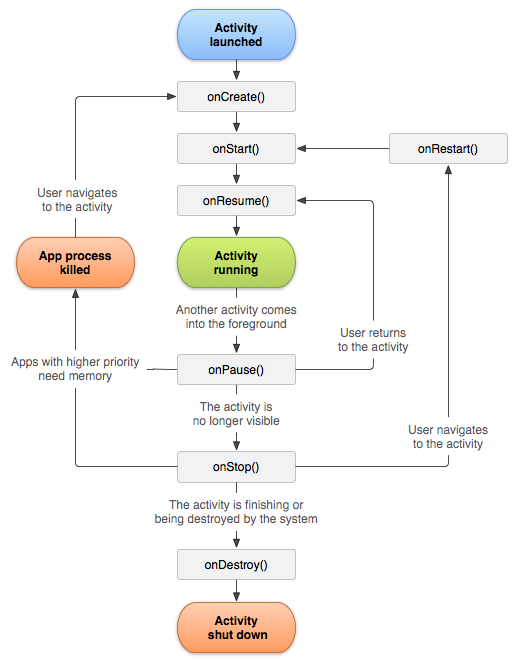
\includegraphics[width=7cm]{developerandroidcom_activitylifecycle.png}
		\caption{Activity lifecycle lånt af developer.android.com}
		\label{fig:android:activities:activitylifecycle}
	\end{center}
\end{figure}

Ovenstående figur viser de forskellige stadier en activity er i, og kan hjælpe til at give et overblik over hvornår de forskellige metoder bliver kaldt, og dermed også hvad man gerne vil have skal ske ide forskellige steps undervejs.

\subsection{Oprettelse af nye activities}

For at oprette en ny activity starter vi med at lave en ny java fil ved siden af MainActivity.java (i ??? folderen) En ny activity skal altid nedarve fra Activity, ligesom MainActivity. 

\begin{example}\noindent
	\begin{JavaCode}{Eksempel på en activity}{pop-up-activity}
		package com.example.housa.myapplication
		
		import android.app.Activity;
		import android.os.bundle;
		
		public class PopUpActivity extends Activity {
		  
		  @Override
		  protected void onCreate(Bundle savedInstanceState) {
		    super.onCreate(savedInstanceState);
		    setContentView(R.layout.activity_popup);
		  }
		}
	\end{JavaCode}
\end{example}

Ud over a skrive selve Java koden der definerer opførslen for en activity skal den til føjes til manifestet. Dette gøres ved at tilføje nedenstående kode til manifestet inde i application tag'et.

\begin{example}\noindent
	\begin{XmlCode}{XML der tilføjer PopUpActivity til manifestet}{add-activity-to-manifest}
		<activity android:name=".PopUpActivity" />
	\end{XmlCode}
\end{example}

For at kunne starte ovenstående activity skal vi benytte os af Intents som vil blive forklaret i næste sektion.


\section{Intents}

En intent er en besked man kan sende for at bede en anden komponent om at gøre noget. Intents kan bruges på flere forskellige måder, men de tre primære brugsscenarier er:

\subsubsection{Starte en anden activity}

Man kan starte en ny instans af en activity ved at sende en intent med som parameter til startActivity(). 

\subsubsection{Starte en service}

En service er et komponent der kører i baggrunden og ikke har noget interface. Man starter en service på lidt samme måde som en activity, nemlig ved at sende en intent med som parameter til metoden startService().

\subsubsection{Sende en broadcast}

En broadcast er en besked som enhver app kan modtage. Der er forskellelige broadcasts for system events som fx foretag opkald eller opladning igang. Man kan sende en broadcast ved at sende en intent med som parameter til sendBroadcast() eller sendOrderesBroadcast().
En standard broadcast kan ikke blive stoppet, og kan ikke videregive resultater. En orderedBroadcast vil sende broadcasten til alle relevante BroadCastRecievers en af gangen og tillade resultatet at propagere.

\subsection{Explicit vs Implicit}

Der er to typer intents explicitte og implicitte. I explicitte intents specificerer man præcist hvilket komponent man vil have til at reagere. Da man kender navngivningen i ens egen app, vil dette være den typeske måde at håndtere kommunikationen indenfor ens egen app, som at starte nye activities inde i appen.

De implicitte intents fortæller ikke præcist hvilket komponent man vil have til at reagere, men i stedet hvilken handling man gerne ville have udført, så kan alle komponenter der har den givne funktionalitet tilbyde at udføre handlingen. Dette benyttes fx hvis man gerne vil have ens app til at sende en mail, men gerne bare vil bruge hvad end mailklient brugeren allerede har på telefonen.

\subsection{Start en activity med en Intent}

hvordan det virker + hvor man gør det henne

eksempel kode

sende beskeder med intents

\subsection{Start en activity fra en anden app med en Intent}

implicit intents

eksempel kode på send mail der benytter indbygget mailklient

\subsection{Start en activity med en Intent fra en anden app}

modtag implicitte intents fra andre apps

broadcastrecievers


\begin{exercise}
	Lav en app der har en main activity, og en anden activity der viser et billede. Tilføj en knap til din main activity, der åbner din anden activity.
\end{exercise}

\begin{exercise}
	Lav en app der har en main activity, og en anden activity med et EditText felt. Tilføj en knap og et EditText felt til din main activity, der åbner din anden activity og viser teksten fra EditText i din main activity.
\end{exercise}

\begin{exercise}
	Lav en Activity der har en ‘send Emil’ knap, der åbner en Email dialog
\end{exercise}

\begin{exercise}
	Lav en activity der agerer som et alternativ til email klienten når man trykker på ‘send mail’ knappen fra opgave 3
\end{exercise}

\begin{exercise}
	Lav en BroadCastReciever, der blokerer alle udgående opkald.
\end{exercise}

\begin{exercise}
	Lav en activity der sender en Broadcast, og en BroadCastReciever der modtager den givne BroadCast.
\end{exercise}

